\documentclass{article}
\usepackage[utf8]{inputenc}
\usepackage{graphicx}
\usepackage{multicol}
\usepackage{amsmath}
\usepackage{titling}
\usepackage[top=2cm,
    		bottom=2cm,
    		left=2cm,
    		right=2cm]{geometry}
\usepackage{algorithm, algpseudocode} % Do not put both alhpseudocode and algorithmic because ovewrite the same command.

\usepackage{booktabs}% for tables

% To gracefully insert code
\usepackage{listings}
\usepackage{xcolor} % for colors

\lstset{
    language=C,                     % set language
    basicstyle=\ttfamily\small,     % font style
    numbers=none,
    %numbers=left,                   % line numbers on the left
    numberstyle=\tiny,              % line number style
    stepnumber=1,                   % number every line
    numbersep=5pt,                  % space between numbers and code
    backgroundcolor=\color{gray!10},% light gray background
    keywordstyle=\color{blue},      % keywords in blue
    commentstyle=\color{green!50!black}, % comments in green
    stringstyle=\color{red},        % strings in red
    breaklines=true,                % allow line breaking
    frame=single,                   % border around code
    tabsize=4                       % tab size
}
%




\usepackage{hyperref}


\graphicspath{{figures/}}



\title{\textbf{Scalability and Communication Overhead in Distributed N-Body Simulation using MPI on GCP}\\}
\author{Claudio Guarrasi\\[1ex]}
\date{%
	\today
	\vspace{-0.25cm}
	\\
	\rule{\textwidth}{0.3pt}}


% Subtitle above title (use \pretitle)
\pretitle{%
  \begin{center}
  	\vspace{-3cm} %vertical distance between upper margin and the logo. A negative value means that I am trying to get them closer.
  	\hspace*{0.1cm} %moving it on the right-
    
\includegraphics[width=0.3\textwidth]{black_unipv_logo_caption_below.png}					\rule{\textwidth}{0.3pt}
    \textit{Advanced Computer Architecture}\\[1ex]
    \Large  % Switch to large font for the title
}
\posttitle{%
	\end{center} % Close centering.
	}

\preauthor{\begin{center}}
\postauthor{%
	\small{Department of Electrical, Computer and Biomedical Engineering}\\
	\small{University of Pavia}\\[1ex]
	\small{Email: \href{mailto:claudio.guarrasi01@universitadipavia.it}{claudio.guarrasi01@universitadipavia.it}}\\
	\small{GitHub: \href{https://github.com/PapiDrago/n-body-problem}{\underline{https://github.com/PapiDrago/n-body-problem}}}
	\end{center}}






\begin{document}
\begin{titlingpage}

\maketitle %thanks to 'titling' package, this command generates also the 'pretitle' and 'posttitle', the 'preauthor' and 'postauthor' and the 'predate' and 'postdate' and put them in the following order: {\pretitle, \title, \posttitle, \preauthor, \author, \postauthor, \predate, \date, \postdate} (\maketitle has been overwritten in the package)
\thispagestyle{empty} % It goes after \maketitle and not after \begin{titlingpage} because \maketitle creates a new page and reset that setting.
\begin{abstract}
This report presents a comprehensive overview of the methods, challenges, and potential solutions involved in the development of a modern technical system. The work includes an analysis of the underlying concepts, a review of relevant literature, and an evaluation of current approaches. Emphasis is placed on both theoretical foundations and practical implementation strategies. The results obtained highlight the effectiveness of the chosen methodology and provide a solid basis for future research or application. This abstract serves as a placeholder and should be replaced with a summary specific to the final version of the report.
\end{abstract}
\end{titlingpage}
\tableofcontents

\thispagestyle{plain}
%\pagenumbering{arabic}

\twocolumn

\section{Introduction}
\label{sec:intro}
The N-body problem is a well-known problem in physics and it has several applications ranging from modeling the gravitational interactions in galaxies and solar systems to simulating charged particle dynamics in plasmas and atoms in molecular systems.

Depending on the goal of the analysis, various assumptions can be relaxed or adjusted. In the experiments I conducted, I considered a closed system of $N$ point masses interacting solely through gravitational forces. This assumption is quite reasonable when modeling astronomical systems, especially when the goal is to compute the trajectories of celestial bodies within them. In such systems, the gravitational force dominates due to the extremely large masses involved, allowing other forces to be safely neglected.

Numerous algorithmic solutions have been proposed to address the N-body problem, many of which have been implemented in software to automate the computation of relevant physical quantities.

This work does not aim to propose a new or improved algorithmic solution. Instead, given an existing approach, the focus is on developing a parallel implementation that highlights the complexities involved in distributing the computation and evaluates its performance in a distributed environment.

Essentially the objectives of this work were:
\begin{enumerate}
\item to analyze a possible serial algorithm for solving the N-body problem;
\item to perform an \emph{a priori} study of the available parallelism using Amdahl's Law;
\item to develop a parallel implementation using the Message Passing Interface (MPI);
\item to evaluate performance and scalability through experiments conducted on Google Cloud Platform (GCP).
\end{enumerate}

\section{Physical Model}
In order to understand the algorithm it is important to recall the physics laws on which the model is based.
\begin{itemize}
\item Newton's law of universal gravitation:
\begin{equation}
\vec{F}_{i,j}=G\frac{m_{i} m_{j}}{\|\vec{r}_{i}-\vec{r}_{j}\|^3}(\vec{r}_{j}-\vec{r}_{i})
\label{eq:gravitation}
\end{equation}
\begin{description}
    \item[\( G \)] Gravitational constant.
    \item[\( m_i, m_j \)] Masses of bodies \( i \) and \( j \).
    \item[\( \vec{r}_i, \vec{r}_j \)] Position vectors of bodies \( i \) and \( j \).
    \item[\( \vec{F}_{i,j} \)] Force acting on body \( i \) due to body \( j \).
\end{description}
Please note that $\vec{F}_{i,j}$ is an attractive force that has the same direction of the displacement vector \mbox{$(\vec{r}_j - \vec{r}_i)$}.
\item Newton's second law of motion:
\begin{equation}
\Sigma\vec{F} = m\vec{a}
\label{eq:motion}
\end{equation}
It states that the sum of all the forces $\Sigma\vec{F}$ acting on a particular point mass is equal to the product between its mass $m$ and its acceleration $\vec{a}$.
\end{itemize}
In our scenario we can combine~\eqref{eq:gravitation} and~\eqref{eq:motion} to obtain, at a certain time instant, the acceleration $\vec{a}_i$ of point mass $i$ implied by all the gravitational forces acting on that point mass. Analytically we can write:
\begin{equation}
\vec{a}_i=\sum_{\substack{j=0 \\ j \neq i}}^{N-1}\left[G\frac{m_j}{\|\vec{r}_i-\vec{r}_j\|^3}(\vec{r}_j-\vec{r}_i)\right]
\label{eq:acceleration}
\end{equation}
Since we are ultimately interested in the trajectory of each body, from $\vec{a}_i$ we can compute the velocity $\vec{v}_i$ and the position $\vec{r}_i$ of mass $i$ by simply integrating $\vec{a}_i$ with respect to time.
\begin{equation}
\vec{v}_i(t_k) = \vec{v}_i(t_{k-1}) + \int_{t_{k-1}}^{t_k} \vec{a}_i(\tau)\, d\tau
\label{eq:continuous_v}
\end{equation}
\begin{equation}
\vec{r}_i(t_k) = \vec{r}_i(t_{k-1}) + \int_{t_{k-1}}^{t_k} \vec{v}_i(\tau)\, d\tau
\label{eq:continuous_r}
\end{equation}
\begin{description}
\item $t_{k-1}$ Time instant defining the initial condition for the current time step.
\end{description}
Although the notation $t_k$ and $t_{k-1}$ may initially appear cumbersome, it will prove useful later when expressing the iterative numerical formulation of the problem.
\subsection{Iterative Nature of the N-body Solution}
It is important to note that for systems involving more than two bodies (\( N > 2 \)), the N-body problem does not admit a general closed-form solution. This means that it is not possible to determine the complete trajectories of all bodies analytically from the initial conditions alone.

In the special case \( N = 2 \), the problem can be reduced to a one-body system by moving to the center-of-mass reference frame. In this frame, the motion can be fully described using relative coordinates, and a closed-form analytical solution can be derived for the position and velocity of each body. However, as soon as a third body is introduced, the system becomes non-linear and highly sensitive to initial conditions, making analytical solutions intractable in the general case~\cite{heggie2005classical}.

For this reason to compute the position of one particular mass at time $k$ it is necessary to iteratively solve the equations of motion (\eqref{eq:acceleration},\eqref{eq:continuous_v},\eqref{eq:continuous_r}) for all the $N$ bodies at each time step $t \leq k$. This is required because, as shown in \eqref{eq:acceleration}, the acceleration at time $k$ depends on the positions of all the bodies at that time.
Just from this consideration we can already anticipate the high computational cost.

\subsection{Numerical Integration}
\label{subsec:num_int}
At each simulation step, we must numerically integrate the equations of motion in order to update the velocity and position of all bodies. In the continuous-time domain, this corresponds to evaluating \eqref{eq:continuous_v} and \eqref{eq:continuous_r}.

However, in practice a digital computer can only work with discrete time instants due to its inherent limitations: it operates at a finite clock frequency, stores only a finite number of samples in memory, and uses finite-precision arithmetic. As a result, we reformulate the problem in the discrete-time domain.

For convenience, the vector notation is omitted here. The time-discretized velocity update equation can be expressed as:
\begin{equation} % '&' is used as alignment point.
\left\{
\begin{aligned}
\frac{v_{k+1}-v_k}{\Delta t} &= a_k(r_k, k) \\
v_k &=v(k \Delta t)
\end{aligned}
\right.
\end{equation}
\begin{description}
\item[$v_k$] Velocity at time $t_k$, with $t_k = k \, \Delta t$.
\item[$a_k(r_k, k)$] Acceleration at step $k$, computed from \eqref{eq:acceleration}.
\item[$\Delta t$] Step size between two consecutive time instants.
\end{description}
With some little algebraic manipulations we can obtain:
\begin{equation}
v_{k+1}=v_k+a_k\Delta t
\label{eq:v_explicit_euler}
\end{equation}
Similarly, the position update is:
\begin{equation}
r_{k+1}=r_k+v_k\Delta t
\label{eq:r_explicit_euler}
\end{equation}
Incidentally, we expressed position and velocity using the explicit Euler method~\cite{atkinson1989introduction}.

However, not all numerical integration methods are equally suitable when simulating physical systems on a computer. This can be seen by writing the exact velocity at time step $k+1$ using the Taylor expansion with Lagrange remainder:
\begin{equation}
\begin{aligned}
v(t_k+\Delta t) = v(t_k) + a(&t_k)\,\Delta t
+ \frac{\Delta t^2}{2} \frac{d^2 v}{dt^2}(\xi), \\
&\qquad \xi \in \left[ t_k,\, t_k+\Delta t \right]
\end{aligned}
\label{eq:v_taylor}
\end{equation}
Neglecting the second-order term yields \eqref{eq:v_explicit_euler}. This highlights that any numerical integration method produces an approximation, and in the case of explicit Euler, the local truncation error is proportional to $\Delta t^2$.

Choosing a very small $\Delta t$ reduces the error but increases the computational cost.
For example, if $\Delta t = 0.01\,\text{s}$, simulating one second of motion requires $100$ iterations of the solution algorithm, whereas with $\Delta t = 0.1\,\text{s}$, only $10$ iterations are needed.

It also crucial to address the fact that, iteration after iteration, the numerical error accumulates, bringing the computed velocity to deviate more and more from the true value, which in turn causes the total energy of the simulated system to drift, violating the thermodynamical principle of energy conservation.
For the N-Body system described in section~\ref{sec:intro}, this can be seen by considering the total kinetic energy $K_{\text{TOT}}$ of the system at time step $k$:
\begin{equation}
K_{TOT}(k) = \frac{1}{2} \sum_{i=0}^{N-1}m_iv_i^2(k)
\end{equation}
Since the system is closed, this quantity should remain constant during the simulation. However, due to the impossibility of computing the exact velocities, this condition cannot be perfectly satisfied.
What can be done instead is to bound the energy oscillations around the true value.
It can be proven that a \emph{symplectic} numerical methods allows us to achieve this~\cite{ENGLE2005432}.

It is for this reason that I chose to pick for my project the \emph{semi-implicit Euler} integration method, which is symplectic \cite{cioaca2013impactexplicitsemiimplicitintegration}, and very similar to explicit Euler method. The only difference is that to compute the position at time step $k+1$ we use the updated velocity $v_{k+1}$ and not the velocity at the previous time step $k$ as seen in \ref{eq:v_explicit_euler}:
\begin{equation}
r_{k+1}=r_k+v_{k+1} \, \Delta t
\label{eq:v_semi_implicit}
\end{equation}

\section{Serial Algorithm}
In the literature~\cite{heggie2005classical}, several approaches have been proposed to address the N-body problem, each with different computational complexities and levels of approximation.  
In this project, the \emph{direct method} was chosen, as it most closely reflects the conceptual formulation of the problem without making further approximations.

Algorithm~\ref{alg:serial} shows the basic structure of the direct method: initially all the $N$ bodies are initialized. Each of them has mass, a starting position and a starting velocity. Then, for each simulation step, the kinematic quantities are updated. 

\begin{algorithm}[H]
\caption{Serial N-body algorithm (direct method)}
\label{alg:serial}
\begin{algorithmic}[1]
\State Initialize positions, velocities, and masses
\For{each time step}
    \State Compute accelerations (Algorithm~\ref{alg:inner_loop})
    \State Update velocities
    \State Update positions
\EndFor
\end{algorithmic}
\end{algorithm}

\subsection{Complexity Analysis}

\subsubsection{Time Complexity}
\label{subsec:time_complexity}
The overall time complexity is dominated by the \emph{Compute accelerations} algorithm~\ref{alg:inner_loop}, since the other components of the serial algorithm involve only a single loop over the $N$ bodies ($N$ is the problem size). In contrast, the \emph{Compute accelerations} step contains a nested loop that also iterates over all $N$ bodies (in practice $N-1$, which is asymptotically equivalent to $N$). 

More precisely, the actual computational cost also depends on the number of time steps $T$ in the simulation, leading to a total complexity of $O(T N^2)$.

Since in the experiments conducted $N \gg T$, the factor $T$ will be omitted from the complexity expressions in the remainder of this work.

\begin{algorithm}
\caption{Inner loop: compute accelerations (direct method)}
\label{alg:inner_loop}
\begin{algorithmic}[1]
\Require Positions $\{\vec r_j\}_{j=0}^{N-1}$, masses $\{m_j\}_{j=0}^{N-1}$
\Ensure Accelerations $\{\vec a_i\}_{i=0}^{N-1}$
\For{$i \gets 0$ to $N-1$}
  \State $\vec a_i \gets (0,0,0)$
  \For{$j \gets 0$ to $N-1$}
    \If{$j \neq i$}
      \State $\vec d \gets \vec r_j - \vec r_i$
      \State $R^3 \gets \|\vec d\|^3 $
      \State $invR^3 \gets 1 /R^3$
      \State $\vec a_i \gets \vec a_i + G \, m_j \, invR^3 \, \vec d$
    \EndIf
  \EndFor
\EndFor
\Statex \textbf{Time complexity:} $O(N^2)$
\end{algorithmic}
\end{algorithm}

\subsubsection{Space Complexity}
The serial algorithm requires storing the masses, the positions, the velocities and the accelerations of the $N$ bodies. Since the kinematic quantities are 3D vectors, each elements corresponds to 3 floating-point values.
This means the total storage is:

This means the total storage is: %align is a math environment
\begin{align*}
&N \ \text{masses} + 3N \ \text{positions} + 3N \ \text{velocities} \\
&\quad + 3N \ \text{accelerations} = 10N \ \text{real values}
\end{align*}

Asymptotically, this results in a space complexity of $O(N)$.  

On modern general-purpose computers, this is not a limiting factor because several gigabytes of RAM are available. For example, if double precision is used (8 bytes per floating-point number), one million bodies would require:
\[
8 \times 10 \times 10^6 = 80 \ \text{MB}
\]
which easily fits in memory.

\subsection{Implementation in C}
\label{subsec:c_impl}
The conceptual serial algorithm described in the previous subsection was implemented in the C programming language. This choice was primarily motivated by the need to perform detailed profiling of the code. The complete source code is publicly available on the GitHub repository for this project\footnote{\url{https://github.com/PapiDrago/n-body-problem}\label{fn:repo}, file \emph{serial.c}}.

The implementation follows closely the structure of Algorithm~\ref{alg:serial}, with each major step of the simulation (initialization, acceleration computation, velocity update, and position update) mapped to dedicated functions.
This modular structure facilitates both readability and profiling, enabling the identification of computational bottlenecks.  

It is worth noticing that to represent the physical vector has been used a struct called \emph{vector} which has three fields, each one is of type \emph{double} and corresponds to one of the three vector components.
In addition the serial application, at the end of each simulation step, prints the positions of all the bodies on a text file. This has been done in order to check qualitatively the resuls and to compare them to those of the MPI parallel application.

\subsubsection{Testing}
Testing was performed qualitatively, leveraging the physical laws embedded in the program’s functions and the results discussed in Subsection~\ref{subsec:num_int} regarding symplectic numerical integrators, which ensure long-term stability of the simulated system.

For this purpose, a slightly modified version of the serial application (\emph{serial\_testing.c}), adapted from~\cite{wiki:n_body}, was used. This variant allows the user to configure simulation parameters, including the number of bodies, the time-step size, and all initial quantities for each body (mass, position, and velocity), via a plain-text input file. The exact file format is documented in the \emph{README.md} of the remote repository.

The application produces an output text file containing the positions of all bodies at each time step. This output was then processed by a Python script (\emph{animate\_nbody\_2d.py}) to generate a 2D animation, enabling a qualitative verification of the trajectories and overall behavior of the simulated system.

Two representative qualitative test cases were examined.  
In the first case, shown in Figure~\ref{fig:two_body_orbit}, the system consisted of a very massive body placed at the origin and a much lighter body with an initial velocity orthogonal to its initial position vector.  
The simulation confirmed the expected physical behavior:  
\begin{itemize}
    \item the massive body remained essentially stationary due to its large inertia,
    \item the lighter body followed a closed orbit (elliptical in this specific setup),
    \item the lighter body’s speed increased when it was closer to the massive body, in agreement with Kepler's second law.
\end{itemize}

\begin{figure}[H]
    \centering
    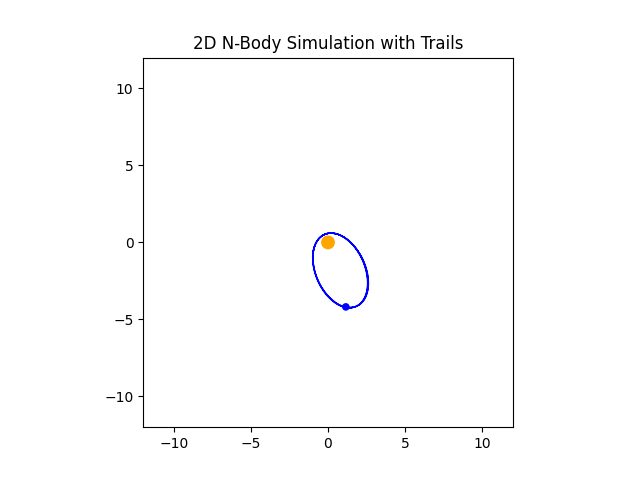
\includegraphics[width=0.6\linewidth]{2_body_orbit.png}
    \caption{Two-body test: a stationary massive body (orange) and a lighter body (blue) in orbit.}
    \label{fig:two_body_orbit}
\end{figure}
The plot in Figure~\ref{fig:two_body_orbit} was obtained by setting the configuation file read by \emph{serial\_testing.c}, as follows:
\begin{itemize}
    \item Body~0 (massive): $m = 1.0$, initial position $(0,0,0)$, initial velocity $(0,0,0)$;
    \item Body~1 (light): $m = 3\times 10^{-6}$, initial position $(-1,-1,0)$, initial velocity $(0,6,0)$.
\end{itemize}
The time step was set to $\Delta t = 0.01$, and the simulation was run for $T=2000$ steps.

A second test was performed using a larger set of bodies, inspired by a simplified solar system model.  
Figure~\ref{fig:long_solar_system} shows the result of a longer simulation run with $T = 2000$ time steps.
\begin{figure}[H]
    \centering
    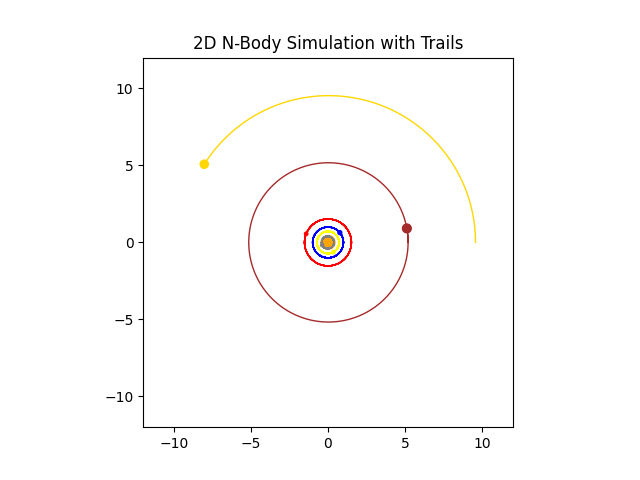
\includegraphics[width=0.6\linewidth]{long_solar_system.png}
    \caption{Solar system test: all the planets revolves steadily around the central star.}
    \label{fig:long_solar_system}
\end{figure}
Throughout the simulation, no planet escaped its orbit, indicating that the numerical integration preserved stability over time.  
Moreover, bodies at different distances from the central mass exhibited the expected orbital periods, and gravitational interactions between planets did not cause unphysical divergence.

These qualitative observations confirm that the combination of the direct gravitational computation and the chosen symplectic integrator (\S\ref{subsec:num_int}) yields a physically plausible evolution, even over longer durations.
  
The parameters used to produce Figure~\ref{fig:long_solar_system} are reported in Appendix~\ref{appendix:solar_params}.

\subsubsection{Random Initialization}
\label{subsec:random_init}
The standard version of the serial application initialized the simulated system randomly. This makes simpler doing experiments with a large quantities of bodies: the program receives the number of bodies from the user through the command-line.
It is worth noticing the use into the inizialization routine of the function \emph{rand\_uniform}.
\begin{lstlisting}
double rand_uniform(unsigned int *seed, double min, double max) {
    return min + (max - min) * ((double)rand_r(seed) / RAND_MAX);
}
\end{lstlisting}
Using a seed allows to have random reproducible inizializations since a seed determines the beginning of the pseudo-random sequence of values and furthermore the calling of \emph{rand\_r(seed)} ensures that each different processes who may running the application use the same seed. The latter will be crucial when comparing the results with the parallel application.
Please also notice that in \emph{rand\_uniform} function we also normalize what \emph{rand\_r(seed)} returns and bounds that number to an arbitrary range and that RNG values are drawn from an uniform distribution in order to avoid directional or positional biases.

In our experiments the interval $\left(-1.0, 1.0\right)$ has been forced to focus on the gravitational interaction.


\subsubsection{Performance Analysis}
\label{subsec:performance_analysis}
In subsection~\ref{subsec:time_complexity}, it was shown that the time complexity of the serial algorithm is $O(N^2)$.  
To evaluate whether this theoretical estimate holds in practice, the C implementation was executed eight times with the number of bodies $N$ increasing from $100$ to $12\,800$.  
For all runs, the number of simulation steps was fixed at $T = 100$, the time step size at $\Delta t = 0.01$, and the gravitational constant at $G = 39.47$.  

Execution time was measured using the \emph{clock} function from the C standard library (\texttt{time.h}).  

The tests were conducted on a machine whose detailed specifications are reported in Appendix~\ref{appendix:machine_specs}.

\begin{figure}[H]
    \centering
    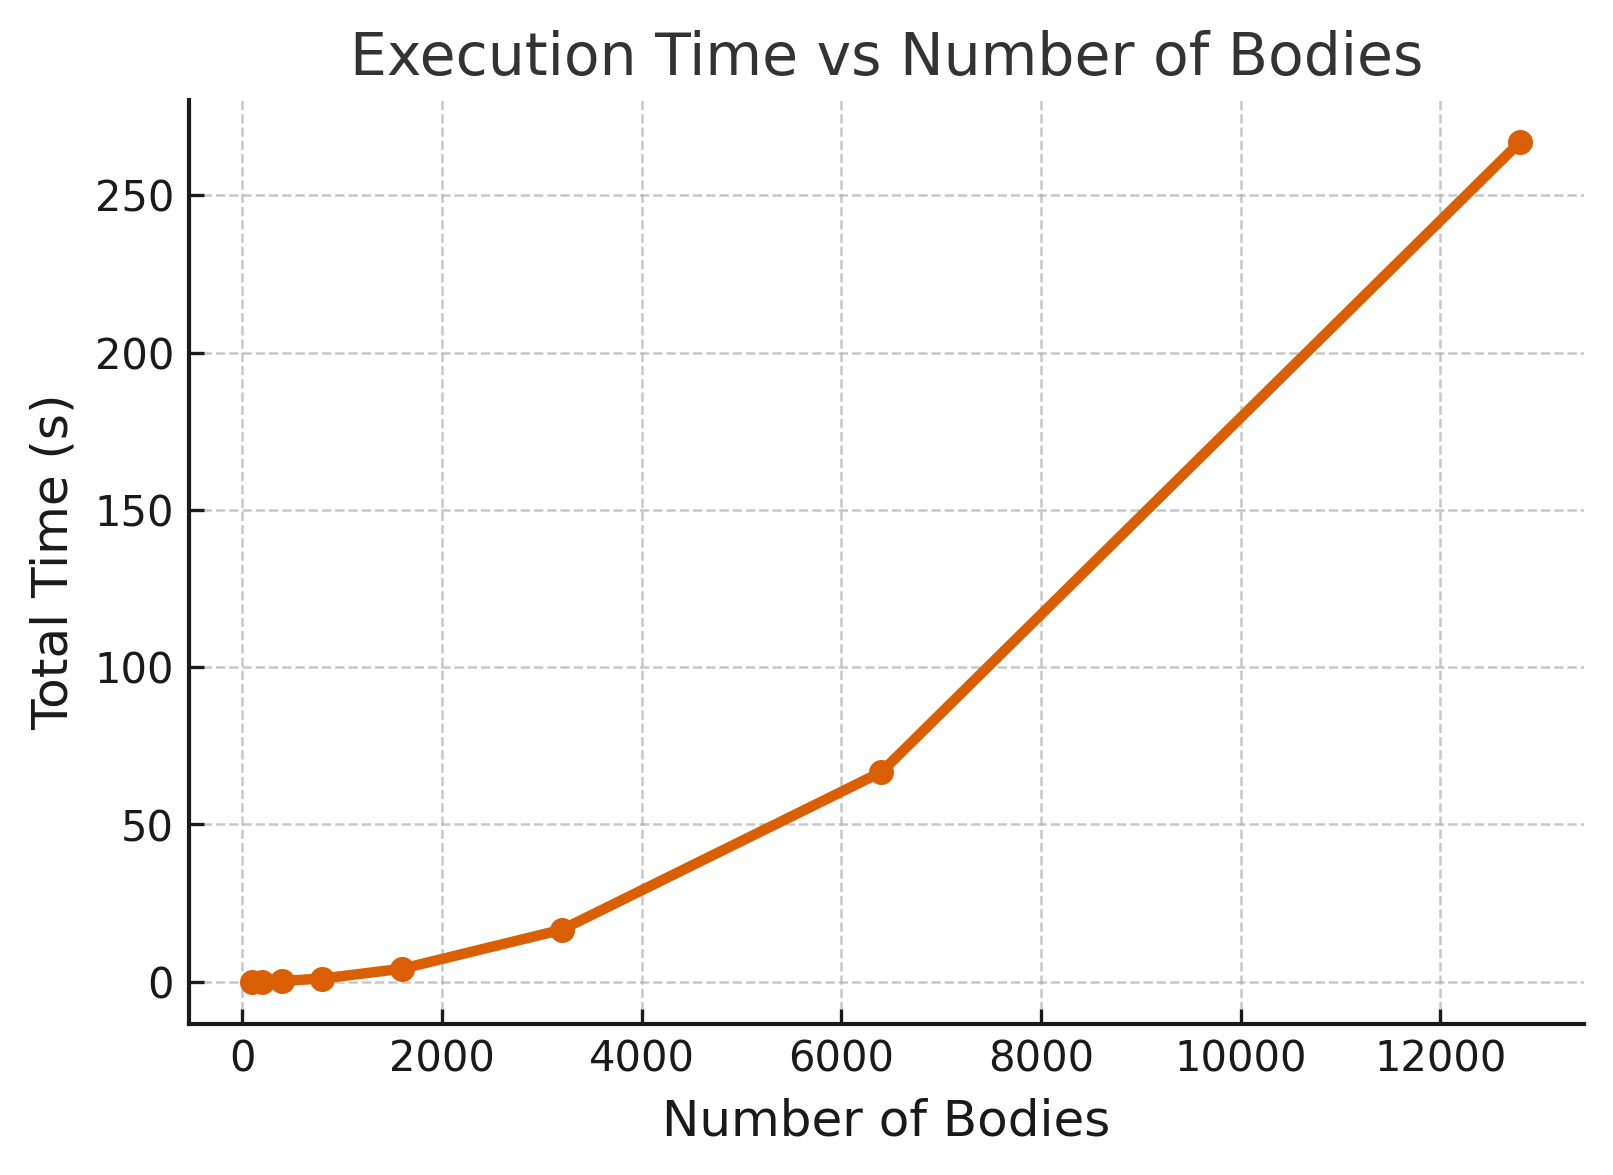
\includegraphics[width=0.6\linewidth]{ex_time_vs_bodies.png}
    \caption{Execution time as a function of the number of bodies $N$.}
    \label{fig:ex_time}
\end{figure}
As expected the running time has a non-linear relationship with the number of bodies as can be seen in Figure \ref{fig:ex_time}.

The log-log plot in Figure \ref{fig:logex_time} reveals an approximately straight line, indicating a power-law relationship, i.e., a quantity varies with the power of another, suggesting a time complexity around $O(N^2)$.

\begin{figure}[H]
    \centering
    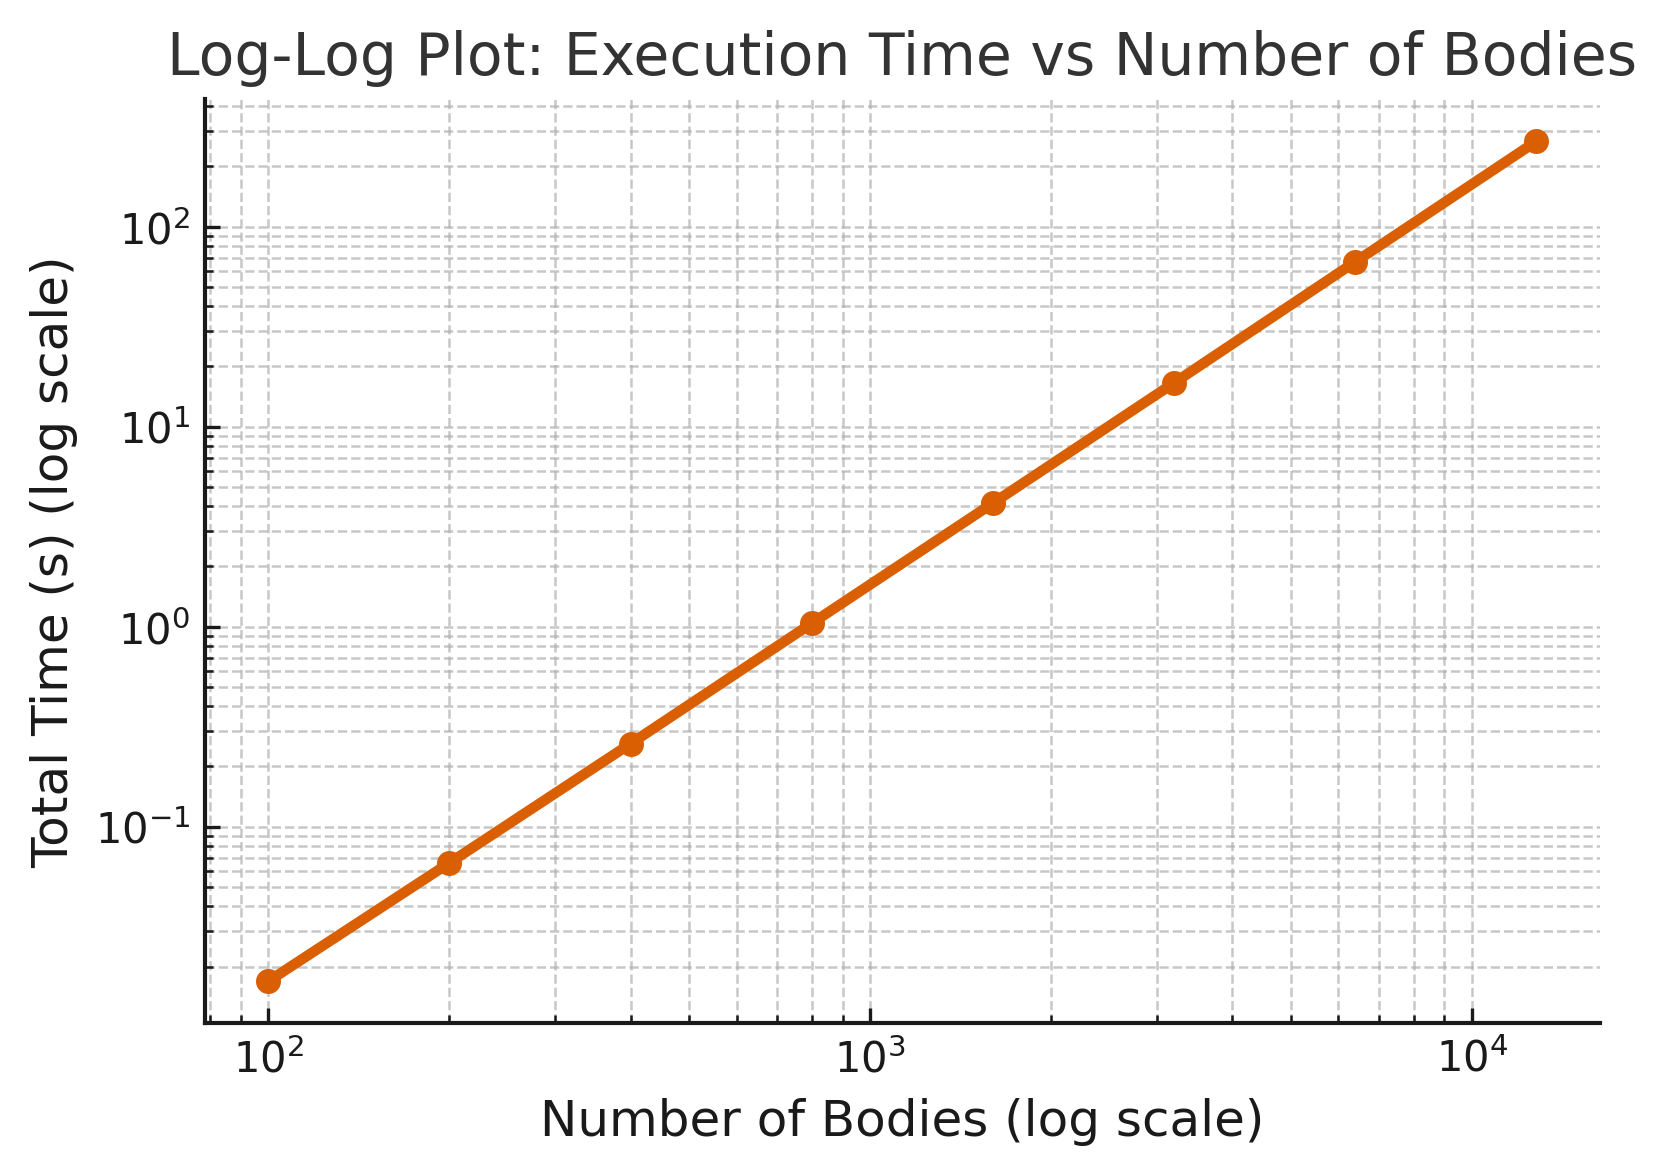
\includegraphics[width=0.6\linewidth]{logex_time_vs_logbodies.png}
    \caption{Log-log plot of execution time vs.\ number of bodies, revealing a power-law relationship.}
    \label{fig:logex_time}
\end{figure}
The raw measurements used to generate Figures~\ref{fig:ex_time} and~\ref{fig:logex_time} are reported in Appendix~\ref{appendix:serial_times}.

Since the empirical results confirmed that the time complexity of the C program is $O(N^2)$, it is worth recalling the reasoning presented in subsection~\ref{subsec:time_complexity}: the overall time complexity is dominated by the \emph{Compute accelerations} algorithm~\ref{alg:inner_loop}, as the other components of the serial algorithm involve only a single loop over the $N$ bodies ($N$ being the problem size).
This implies that the execution time is mainly due to the \texttt{compute\discretionary{}{}{}Accelerations()} function.

To verify this, the C code was compiled with profiling enabled, and the \emph{gprof} profiler 
was used to produce a performance report. The main results are presented in 
Appendix~\ref{appendix:gprof_results}.
As predicted, \texttt{computeAccelerations()} dominates the runtime (98.49\%), confirming it is the primary bottleneck of the serial implementation.

It is also insightful to analyze performance from a hardware perspective. The built-in Linux profiler \emph{perf} was used for this purpose.
The results of the \emph{perf} profiler are reported in Appendix~\ref{appendix:perf_results}.

Since \texttt{compute\discretionary{}{}{}Accelerations()} keeps the CPU busy for the vast majority of execution time, these measurements can be safely attributed to this function.

The very low branch-miss rate ($0.06\%$) indicates that the control flow within the inner loop is highly predictable. Furthermore, the low percentage of frontend idle cycles ($0.14\%$) confirms that the workload is highly CPU-bound.
The measured instructions-per-cycle (IPC) of $2.43$ corresponds to a cycles-per-instruction (CPI) of approximately $0.41$, meaning that on average each instruction is retired in less than one clock cycle. This is likely due to the microarchitecture of the test machine, which can exploit multiple execution pipelines, out-of-order execution, minimal memory stalls and compiler optimizations.

\subsubsection{A-priori Study of Available Parallelism}
\label{subsec:apriori_parallelism}
In Subsection~\ref{subsec:performance_analysis} it is highlighted how, although the \texttt{compute\discretionary{}{}{}Accelerations()} is the bottleneck of the serial algorithm, its CPI is ($0.41$), which is lower than 1.
This efficiency is due both to the microarchitecture of the testing machine (see Appendix~\ref{appendix:machine_specs}) and to the limited data dependencies in 
\texttt{compute\discretionary{}{}{}Accelerations()}, namely that to compute the accelerations, 
only the positions need to be known in advance.

On the other hand is crucial to note that the inner loop (Algorithm~\ref{alg:inner_loop}) iterations are independent from one another, i.e., they could be overlapped.
This means, of course, that loop unrolling can be applied, but more importantly that the loop iterations can be distributed across processes.

This suggests that it would be effective to build a parallel application.
By using \emph{Amdahl’s law} it is possible to know a priory the theoretical speedup of the parallel application, i.e., how much faster the parallel program would be compared to the serial algorithm.
\begin{equation}
\begin{aligned}
Speedup(N) &= \frac{time_{serial}}{time_{parallel}(N)}=\frac{(S+P)\times time_{serial}}{(S\times t_{serial}+\frac{P\times t_{serial}}{N})} \\ &=\frac{S+P}{S+\frac{P}{N}}=\frac{1}{S+\frac{P}{N}}
\end{aligned}
\label{eq:amdahl}
\end{equation}
\begin{description}
    \item[\normalfont{$time\_{serial}$}] Execution time of the serial application.
    \item[\normalfont{$time\_{parallel}$}] Execution time of the parallel application.
    \item[\normalfont{$N$}] The number of CPUs.
    \item[\( S \)] The fraction of the code that cannot be parallelized (inherently sequential part).
    \item[\( P \)] The fraction of the code that can be parallelized.
    \item[\( S + P = 1 \)].
\end{description}
In this case all the code can be parallelized since there are no loop-carried dependencies. Nevertheless also the other pieces of the program can be parallelized as well.
Then applying~\eqref{eq:amdahl}, with $S=0$ and $P=1$, gives:
\begin{equation}
Speedup(N)=N
\label{eq:speedup}
\end{equation}
This means that a priori a linear speedup is expected: doubling the number of CPUs $N$ corresponds to halve the execution time.
\begin{figure}[H]
    \centering
    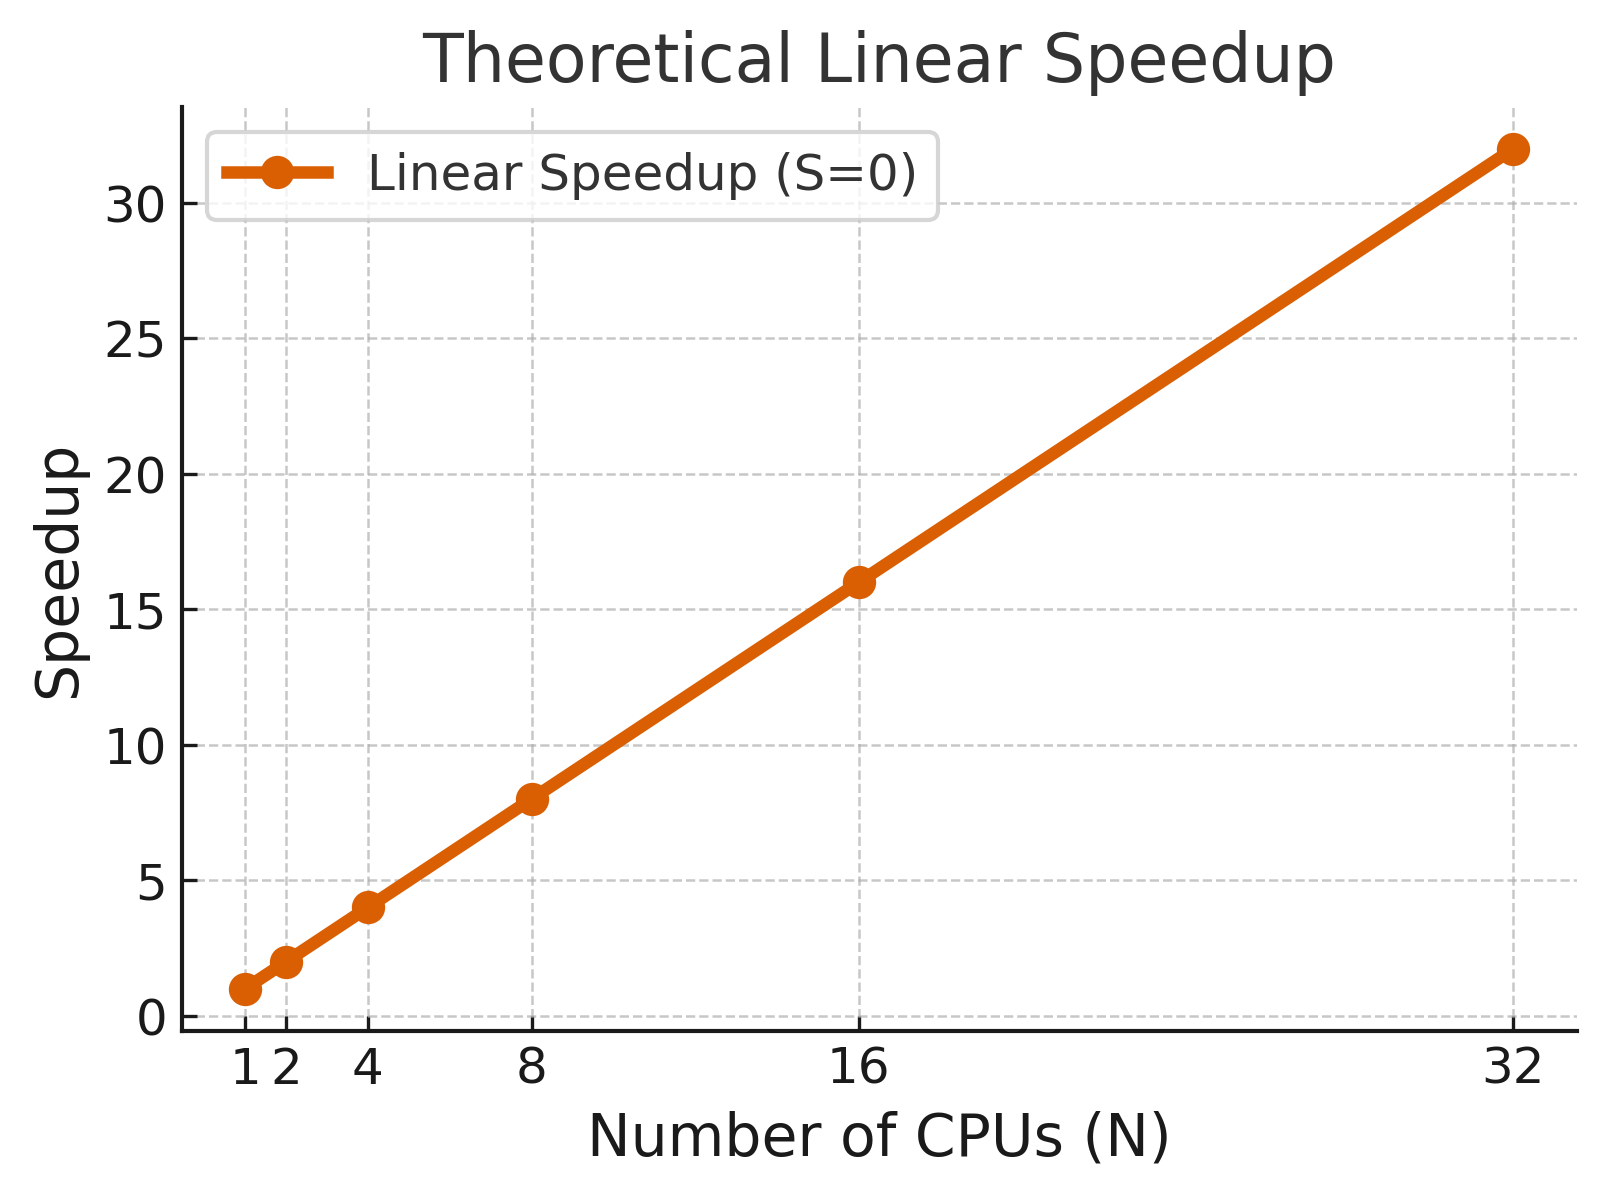
\includegraphics[width=0.6\linewidth]{linear_speedup.png}
    \caption{Speedup as a function of the number of CPUs.}
    \label{fig:linear_speedup}
\end{figure}
However, this scenario is too optimistic to be true — and indeed it would only occur if communication among the processes were instantaneous. To be clear if we assign to each CPU (process) a single mass, in order for each process to compyte the acceleration for its own mass it is necessary to know where the other masses are located. Hence each process has to communicate the other the position and this takes time.

\section{Parallel Algorithm}
\subsection{Conceptual Design}
The chosen approach to parallelize the N-body problem algorithm (Algorithm~\ref{alg:serial}) is as follows.  
Given $N$ bodies and $P$ processes, each process is assigned $\frac{N}{P}$ bodies.  
This means it is responsible for initializing these bodies and updating their kinematic quantities during the simulation.  

However, to compute the accelerations for its local bodies, a process requires the positions of \emph{all} bodies in the system.  
For this reason, after the initialization phase and at the end of every simulation step, all processes must exchange the positions of their bodies.  
During the initialization phase, the masses must also be broadcast to all processes, since they are required in the acceleration computation.
It is important to note that no process can start computing accelerations for its local bodies until it has received the position data from all other processes.
This flow is shown in Algorithm~\ref{alg:parallel}.

\begin{algorithm}[H]
\caption{Parallel N-body (single-process view)}
\label{alg:parallel}
\begin{algorithmic}[1]
\State Initialize local positions, local velocities, and local masses
\State Send local positions and local masses
\State Wait for global positions and global masses
\For{each time step}
    \State Compute local accelerations (Algorithm~\ref{alg:parallel_inner_loop})
    \State Update local velocities
    \State Update local positions
    \State Send local positions
    \State Wait for global positions
\EndFor
\end{algorithmic}
\end{algorithm}

As discussed in Subsections~\ref{subsec:performance_analysis} and~\ref{subsec:apriori_parallelism}, 
the main motivation for building a parallel algorithm was to distribute the workload of the inner loop 
of the serial algorithm (Algorithm~\ref{alg:inner_loop}).

Conceptually, the structure of the computation remains the same, with the only difference that 
the outermost loop now iterates over $\frac{N}{P}$ local bodies, as shown in 
Algorithm~\ref{alg:parallel_inner_loop}.


\begin{algorithm}[H]
\caption{Parallel inner loop: compute local accelerations}
\label{alg:parallel_inner_loop}
\begin{algorithmic}[1]
\Require Global positions $\{\vec r_j\}_{j=0}^{N-1}$, global masses $\{m_j\}_{j=0}^{N-1}$
\Ensure Local accelerations $\{\vec a_i\}_{i=0}^{(N/P)-1}$
\For{each local body $i$}
  \State $\vec a_i \gets (0,0,0)$
  \For{$j \gets 0$ to $N-1$}
    \If{$j$ is not the same as global index of $i$}
      \State $\vec d \gets \vec r_j - \vec r_i$
      \State $R^3 \gets \|\vec d\|^3$
      \State $invR^3 \gets 1 / R^3$
      \State $\vec a_i \gets \vec a_i + G \, m_j \, invR^3 \, \vec d$
    \EndIf
  \EndFor
\EndFor
\Statex \textbf{Time complexity (per process):} $O\!\left(\frac{N}{P} \cdot N\right) = O\!\left(\frac{N^2}{P}\right)$
\end{algorithmic}
\end{algorithm}

It follows that the total computational work remains $O(N^2)$, but the per-process 
workload is reduced to $O\!\left(\frac{N^2}{P}\right)$, assuming perfect load balancing 
and negligible communication overhead.

\subsection{Theoretical Scalability}
\label{subsec:theoretical_scalability}
\emph{Scalability} measures how much faster a parallel algorithm runs using P processes compared to running on a single process:
\begin{equation}
Scalability(P) = \frac{t_{parallel}(1)}{t_{parallel}(P)}
\label{eq:scalability}
\end{equation}
where $t_{parallel}(P)$ is the execution time of the parallel application using $P$ processes.


Assuming no communication overhead and ignoring hardware-related effects, in the problem considered in this report, with $P = 1$, the running time can be expressed as
\begin{equation}
t_{{parallel}}(1) = N_1^2 \, \bar{t}
\end{equation}
where $\bar{t}$ is the time per iteration of the inner loop (Algorithm~\ref{alg:inner_loop}) and $N_1$ is the number of bodies in the parallel application with 1 process.

This implies that with $P>1$ the running time is
\begin{equation}
t_{{parallel}}(P) = \frac{N_p^2}{P} \, \bar{t}
\end{equation}
where $N_p$ is the number of bodies in the parallel application with $P$ processes.

Then it is possible to write:
\begin{equation}
Scalability(P) = \frac{N^2_1\bar{t}}{\frac{N_p^2}{P}\bar{t}} = \frac{N_1^2}{N_p^2}P
\end{equation}

Depending on whether the problem size, the total number of bodies $N$, is fixed or increases with $P$, two kinds of scalability measures are typically considered: \emph{strong scalability} and \emph{weak scalability}, discussed below.

\paragraph{Strong Scalability.}
Strong scalability measures how the execution time decreases when the number of processes $P$ increases, while keeping the total problem size $N$ fixed.  
In this case, $N_p = N_1 = N$ and the scalability formula reduces to
\[
Scalability_{\text{strong}}(P) = P
\]
Theoretically, the strong scalability of the parallel N-Body algorithm is ideal, since the same workload can be completed $P$ times faster.
The last equation highlights the fact in this case (direct-method N-body implementation) since there is no inherently sequential part as concluded in Subsection~\ref{subsec:apriori_parallelism}, analyzing strong scalability is essentially equivalent to analyzing speedup.

\paragraph{Weak Scalability.}
Weak scalability measures how the execution time changes when the number of processes $P$ increases while keeping the \emph{per-process workload} fixed.  
Since the per-process workload is $\tfrac{N_p}{P} = N_1$, the scalability formula becomes
\[
Scalability_{\text{weak}}(P) = \frac{N_1^2}{(P N_1)^2} \, P = \frac{1}{P}.
\]

This shows that the presented parallel N-Body algorithm exhibits poor weak scalability.  
Ideally, increasing both the number of bodies $N$ and the number of processes $P$ in the same ratio should maintain the execution time constant, i.e.\ $Scalability_{\text{weak}}(P) = 1$.  
However, this is not the case here: if both $N$ and $P$ are doubled, each process is still responsible for the same number of bodies as before, but the inner loop of the \texttt{compute\discretionary{}{}{}Accelerations()} routine must iterate over all $N$ bodies.  
This can also be seen directly from the per-process time complexity $O\!\left(\tfrac{N^2}{P}\right)$: doubling both $N$ and $P$ results in a doubling of the per-process time.

As a consequence, the per-process workload grows with $P$, and the overall execution time of the parallel algorithm increases rather than staying constant.  
This is an inherent limitation of the direct method formulation in the N-Body problem.


\subsection{MPI Implementation}

The \emph{Message Passing Interface} (MPI) is a standardized specification for developing parallel programs that execute across multiple processes, potentially on different machines~\cite{mpi_standard}.
MPI provides mechanisms for processes to communicate by sending and receiving messages, as well as for synchronizing their execution.
For this project, version~4.1.1 of the \emph{OpenMPI} implementation was used, targeting the C/C++ programming languages~\cite{openmpi_docs}.

The full MPI implementation is provided in the file \texttt{parallel.c}, available in the remote repository associated to the project (see footnote~\ref{fn:repo}).

\subsubsection{Communication Strategy}

With reference to Algorithm~\ref{alg:parallel_inner_loop}, each process requires access to the positions (and initially also the masses) of all bodies in the system in order to compute local accelerations.  
This necessitates both communication and synchronization between processes at each iteration.

In this work, the \texttt{MPI\_Allgatherv} function was chosen for this purpose, since it simultaneously performs the required \emph{sending}, \emph{receiving}, and implicit \emph{waiting}.  
The main advantages are:
\begin{itemize}
    \item \textbf{Blocking collective communication:} every process broadcasts its local data to all other processes in the MPI communicator, ensuring that all participants have a consistent global view. Since the operation is blocking, no process can proceed until the data exchange of all processes has completed;
    \item \textbf{Consistent ordering:} the received items are gathered into arrays, with the same element order from the perspective of each process;
    \item \textbf{Flexibility:} unlike \texttt{MPI\_Allgather}, the \texttt{MPI\_Allgatherv} variant allows each process to contribute a different number of items, which makes it more general and adaptable.
\end{itemize}

The \texttt{MPI\_Allgatherv} function is invoked as follows.
\begin{lstlisting}
MPI_Allgatherv(local_positions, b, MPI_VECTOR, global_positions, recvcounts, displs, MPI_VECTOR, MPI_COMM_WORLD);
\end{lstlisting}
The address of the first element of the sending buffer is represented by \emph{local\_positions}. This buffer has \emph{b} elements where b is the number of bodies each process has to manage.
These elements are of type \emph{MPI\_VECTOR}, a properly defined MPI data type to wrap the struct \emph{vect} already mentioned in Subsection~\ref{subsec:c_impl}.
\begin{lstlisting}
void createVectorType() {
    int count = 3; // Custom MPI_Datatype will have 3 fields (x, y, z)
	int blocklengths[3] = {1, 1, 1}; // Each field is just one element
	MPI_Aint offsets[3]; // How elements in the struct are stored.
    offsets[0] = offsetof(vector, x); // 0 byte offset from struct base as the 'vector' struct
    offsets[1] = offsetof(vector, y); // 8 byte
    offsets[2] = offsetof(vector, z); // 16 byte
    MPI_Datatype types[3] = {MPI_DOUBLE, MPI_DOUBLE, MPI_DOUBLE}; // Each element of custom MPI_Datatype is an MPI_DOUBLE

    MPI_Type_create_struct(count, blocklengths, offsets, types, &MPI_VECTOR);
    MPI_Type_commit(&MPI_VECTOR); // MPI finalizes the definition and use it
}
\end{lstlisting}
This allows the positions (represented as 3D vectors) to be handled and sent in a clear and structured manner.

The array \emph{recvcounts} contains as many entries as the number of MPI processes, since it tells the \texttt{MPI\_Allgatherv} function how many elements each process contributes.
When the number of bodies cannot be evenly divided among processes, the remainder $r$ is distributed in a round-robin fashion: the first $r$ processes each receive one additional body.
This works because MPI assigns each process in the communicator a unique \emph{rank}, from $0$ to $P-1$ (with $P$ the total number of processes).
Consequently, the first $r$ elements of the \emph{recvcounts} array will be incremented by one compared to the others.

The array \emph{displs} is used to ensure that the receiving buffer \emph{global\_positions} is properly organized, i.e., to specify at which offset the data received from each process should be stored.
More precisely, the value at index $i$ indicates the starting position in the receiving buffer where the block of elements broadcast by the process of rank $i$ will be placed. The displacement depends on both the number of elements contributed by each process and the rank order.
The following code shows how both \emph{recvcounts} and \emph{displs} are populated:
\begin{lstlisting}
void computeAllGathervParams(int* recvcounts, int* displs, int size, int q, int r) {
  for (int i = 0; i < size; i++) { /**q = bodies / size, r = bodies % size;**/
      if (i < r) {
         recvcounts[i] = q + 1;
         displs[i] = i * (q + 1);
     } else {
        recvcounts[i] = q;
        displs[i] = r * (q + 1) + (i - r) * q;
    }
  }
}
\end{lstlisting}

\paragraph{Memory remark.}
This communication strategy requires each process to store not only its local data ($3\frac{N}{P}$ positions, $3\frac{N}{P}$ velocities, $3\frac{N}{P}$ accelerations, and $\tfrac{N}{P}$ masses) but also the global arrays ($3N$ positions and $N$ masses).  
This results in a per-process memory usage of
\[
M(P) = 10\frac{N}{P} + 4N,
\]
which asymptotically remains $O(N)$, dominated by the replicated global arrays.
Consequently, memory requirements do not scale down with the number of processes.

\subsubsection{Initialization and Testing}
The initialization phase in the parallel application closely follows what was discussed for the serial application in Subsection~\ref{subsec:random_init}, with the key difference that the seed of the random number generator is not determined solely by the local loop index $i$. Instead, it also depends on the global index of each body.
As a consequence, the initial configuration of the parallel application can be made identical to that of the serial application because the evaluation of the global index reflects the ordered distribution of bodies across processes, mirroring the indexing scheme of the serial application.
 
This reproducibility allows a direct comparison of the outputs, which is essential for validating the correctness of the parallel algorithm.

The global index of the first body managed by each process is computed as follows:
\begin{lstlisting}
unsigned int global_start_index(int r, int bodies, int rank){
    unsigned int start_index;
    if (rank < r) {
      return rank*bodies;
    } else {
      return r*(bodies+1) + (rank - r)*bodies;
      }
}
\end{lstlisting}
Then, during the initialization loop, the seed used for the local body $i$ is set as:
\begin{lstlisting}
unsigned int seed = start_index + i;
\end{lstlisting}

To practically compare the results a simple C program (\texttt{tester.c}) has been used.
When it runs it opens both the output files of the serial and the parallel applications and checks value by value if they are equal within a tolerance introduced to allow the comparison between machines with different floating-point precisions.

\subsection{Experimental Evaluation on GCP}
In order to analyze the performance of the MPI implementation, it was necessary not only to rely on a multi-core architecture capable of running multiple processes concurrently, but also to distribute these processes across different machines in order to assess the impact of inter-process communication through MPI functions—in this case, \texttt{MPI\_Allgatherv}.  

To meet both requirements, multiple virtual instances were deployed on the Google Cloud Platform (GCP), using the Compute Engine service~\cite{gcp_compute}, which allows the creation and execution of virtual machines on Google’s infrastructure.

These virtual instances were organized into experimental clusters, based on their hardware configuration and geographic location:

\begin{itemize}
    \item \textbf{Single fat instance:} 1 machine with 16~vCPUs and 32~GB RAM, located in a single region (us-central1-a).
    \item \textbf{Inter-regional fat instances:} 2 machines with 8~vCPUs and 16~GB RAM each (16~vCPUs total), distributed across two regions: us-central1-a and europe-west9-a.
    \item \textbf{Intra-regional thin instances:} 4 machines with 3~vCPUs and 3~GB RAM each (12~vCPUs total), located in the same region (us-central1-a).
    \item \textbf{Inter-regional thin instances:} 4 machines with 3~vCPUs and 3~GB RAM each (12~vCPUs total), distributed across two regions: us-central1 and europe-west1.
    \item \textbf{Four-region thin instances:} 4 machines with 3~vCPUs and 3~GB RAM each (12~vCPUs total), distributed across four regions: us-central1, europe-west1, asia-northeast1, and me-central1.
\end{itemize}

All experiments carried out on GCP were constrained by the fact that the Google account used had a limited quota of 32~vCPUs across all regions.
The raw data of the GCP experiments can be consulted in Appendix~\ref{appendix:gcp_data} where it is also presented the methodology used to obtain them.

\paragraph{Remark.}  
All the above machines provide two hardware threads per physical core.  
Therefore, in principle, each configuration could run with up to twice as many MPI processes (e.g., 32 processes on the single fat instance instead of 16).  
However, in this work only one MPI process per physical core was used in order to focus on the impact of \emph{network communication overhead}.  
Exploiting both hardware threads would introduce additional effects related to context switching, shared cache contention, and memory bandwidth limitations, which would make it harder to isolate the contribution of inter-process communication.

\subsubsection{Strong Scalability Analysis}
As discussed in Subsection~\ref{subsec:theoretical_scalability}, in this project strong scalability is effectively equivalent to speedup, since the parallel application with a single process can be regarded as the serial application and no inherently sequential part exists in the algorithm.  
Therefore, in the following analysis the terms \emph{speedup} and \emph{strong scalability} will be used interchangeably.
In Subsection~\ref{subsec:apriori_parallelism}, the theoretical speedup was formulated using Amdahl's law, and it was concluded to be ideal since it scales linearly with the number of processes $P$ (Equation~\eqref{eq:speedup}).  
However, it was also anticipated that the overhead introduced by communication through the network could significantly reduce the practical performance.

When increasing the number of processes while remaining on the same machine, the experimental results empirically confirm the theoretical analysis, as shown in Figure~\ref{fig:strong_scaling_single_fat_instance} for the single fat instance.  
In this configuration, the execution time of the parallel application halves when the number of processes is doubled (Figure~\ref{fig:single_fat_instance_ex_time}).

\begin{figure}[H]
    \centering
    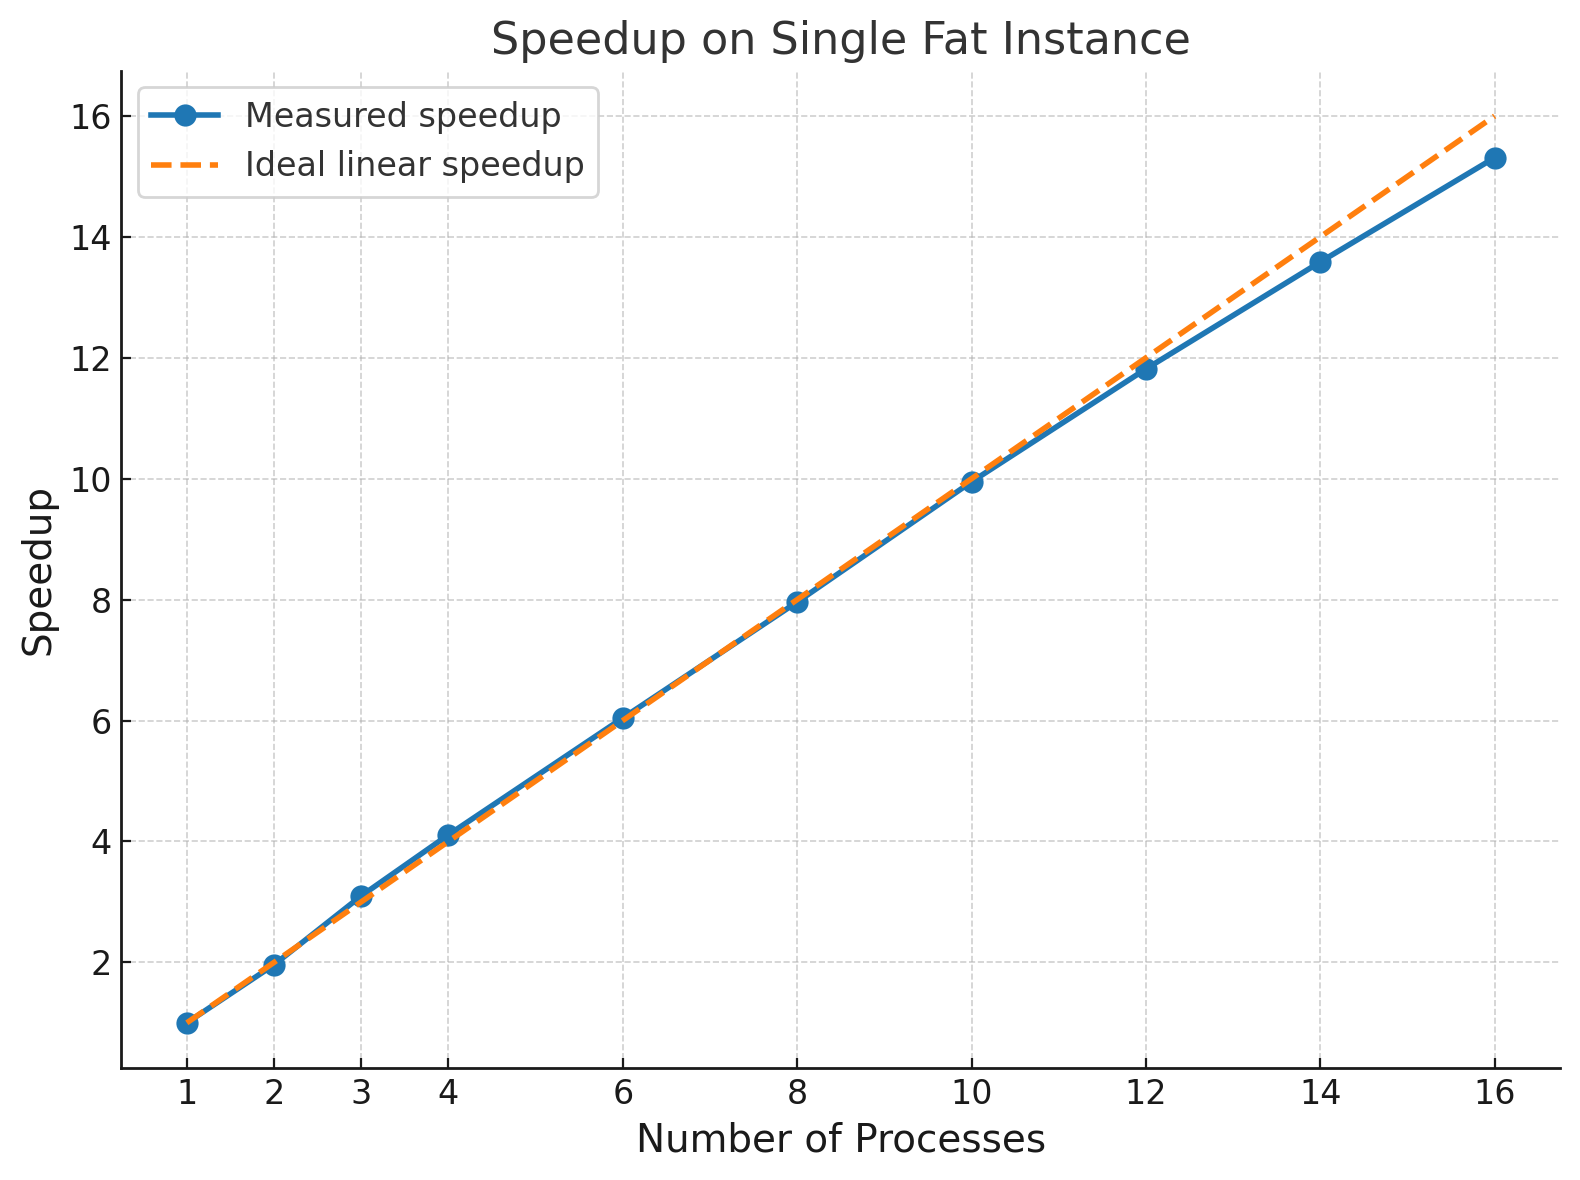
\includegraphics[width=0.8\linewidth]{parallel_strong_scaling_16_cores.png}
    \caption{The single fat instance exhibits good strong scalability.}
    \label{fig:strong_scaling_single_fat_instance}
\end{figure}

\begin{figure}[H]
    \centering
    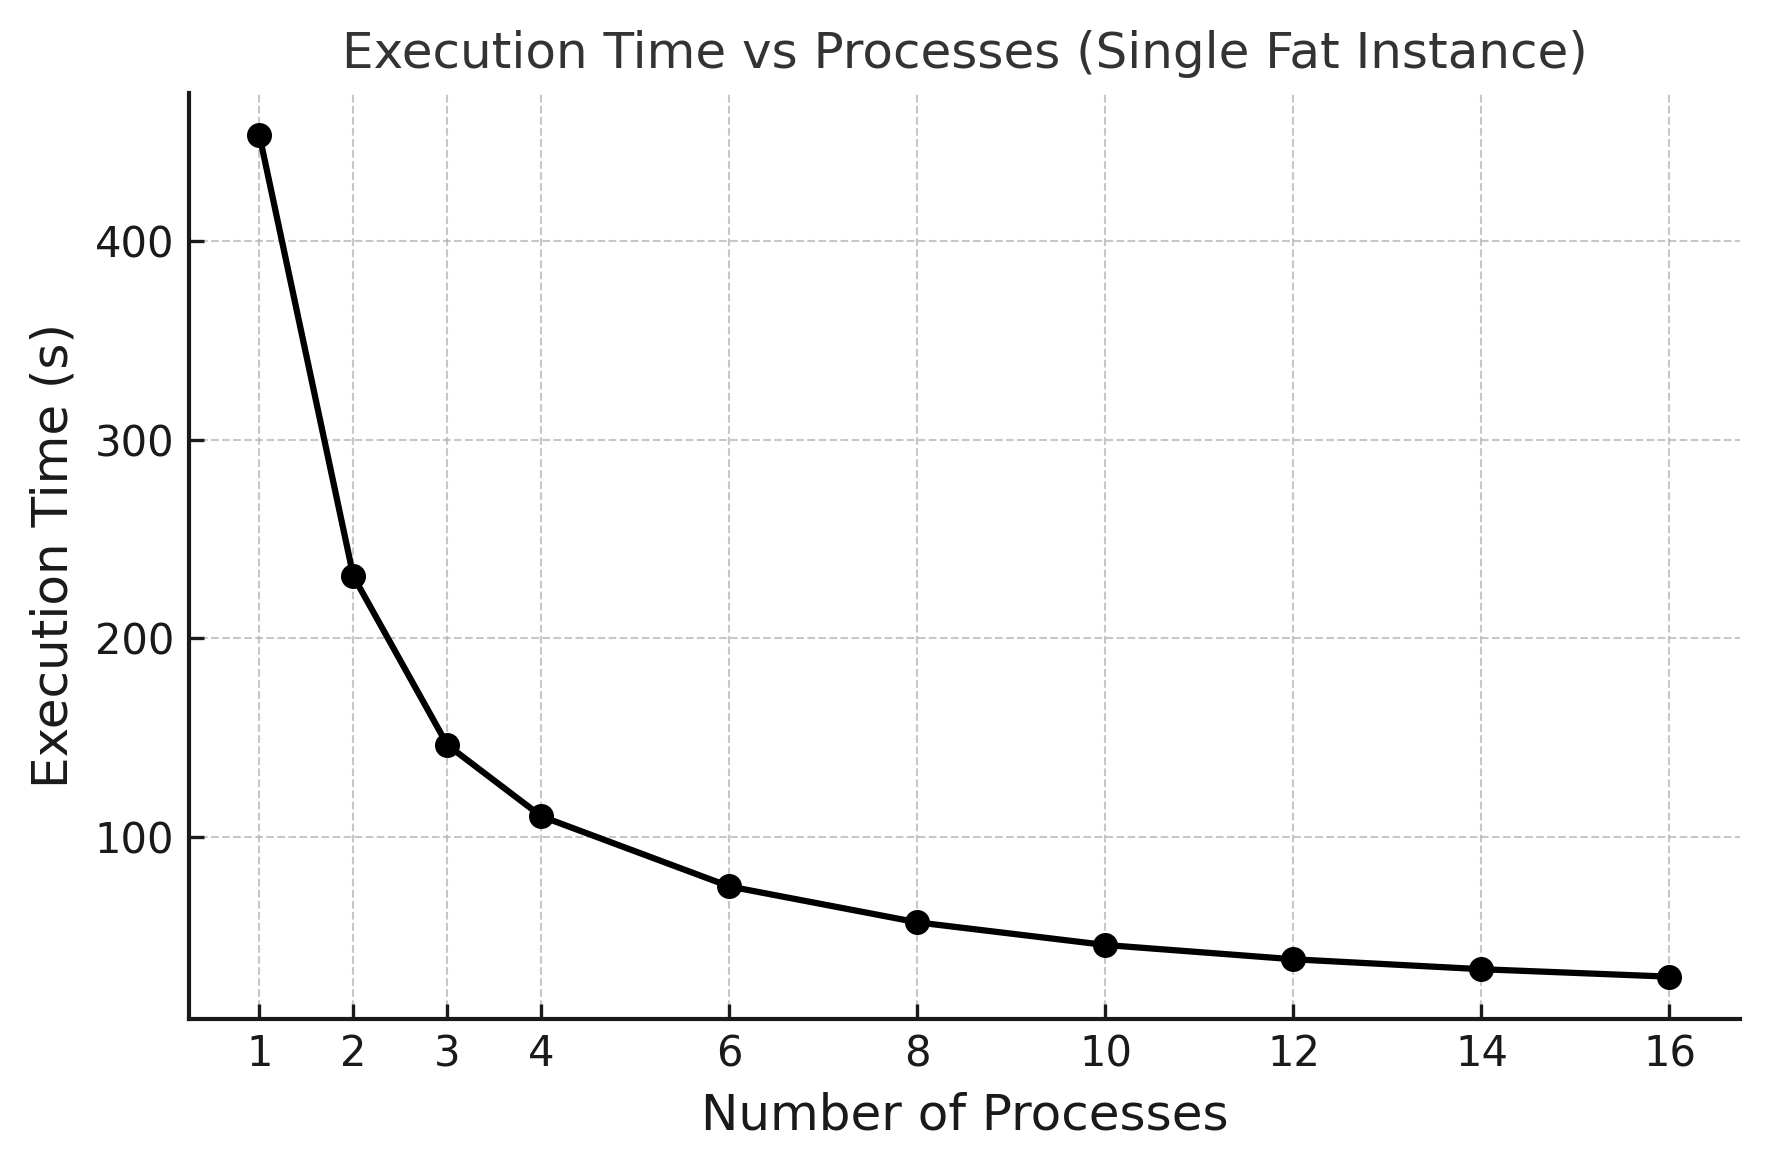
\includegraphics[width=0.8\linewidth]{single_fat_instance_ex_time.png}
    \caption{On the single fat instance, the running time halves each time the number of processes is doubled.}
    \label{fig:single_fat_instance_ex_time}
\end{figure}

The raw measurements used to generate Figures~\ref{fig:single_fat_instance_ex_time} and~\ref{fig:strong_scaling_single_fat_instance} are reported in Appendix~\ref{appendix:gcp_data}.  
These data also show that the total time spent in communication, i.e.\ the cumulative time of \texttt{MPI\_Allgatherv}, remains relatively stable across all executions and is negligible compared to the total running time in this configuration, as illustrated in Figure~\ref{fig:comparison_fraction_communication}. 
Consequently, the achievable speedup of these configurations worsens significantly, as clearly observed in the execution times of the four-region cluster (Figure~\ref{fig:four_region_ex_time}).
This degradation can be explained by the fact that \texttt{MPI\_Allgatherv} is a blocking collective operation: all participating processes must wait until every process has both sent and received its portion of data.
When processes are distributed across geographically distant regions, the overall execution time becomes constrained by the slowest communication path. Thus, even if most processes complete their transfers quickly, a single high-latency or congested link can stall the entire computation, amplifying the communication overhead. Furthermore, it is important to point out that delays due to network latency and throughput are inherently unpredictable. For this reason, Figure~\ref{fig:four_region_ex_time} should not be interpreted as a precise measure of running time, but rather as evidence that—even when increasing the number of processes—it cannot be guaranteed that the execution time will decrease.

\begin{figure}[H]
\centering
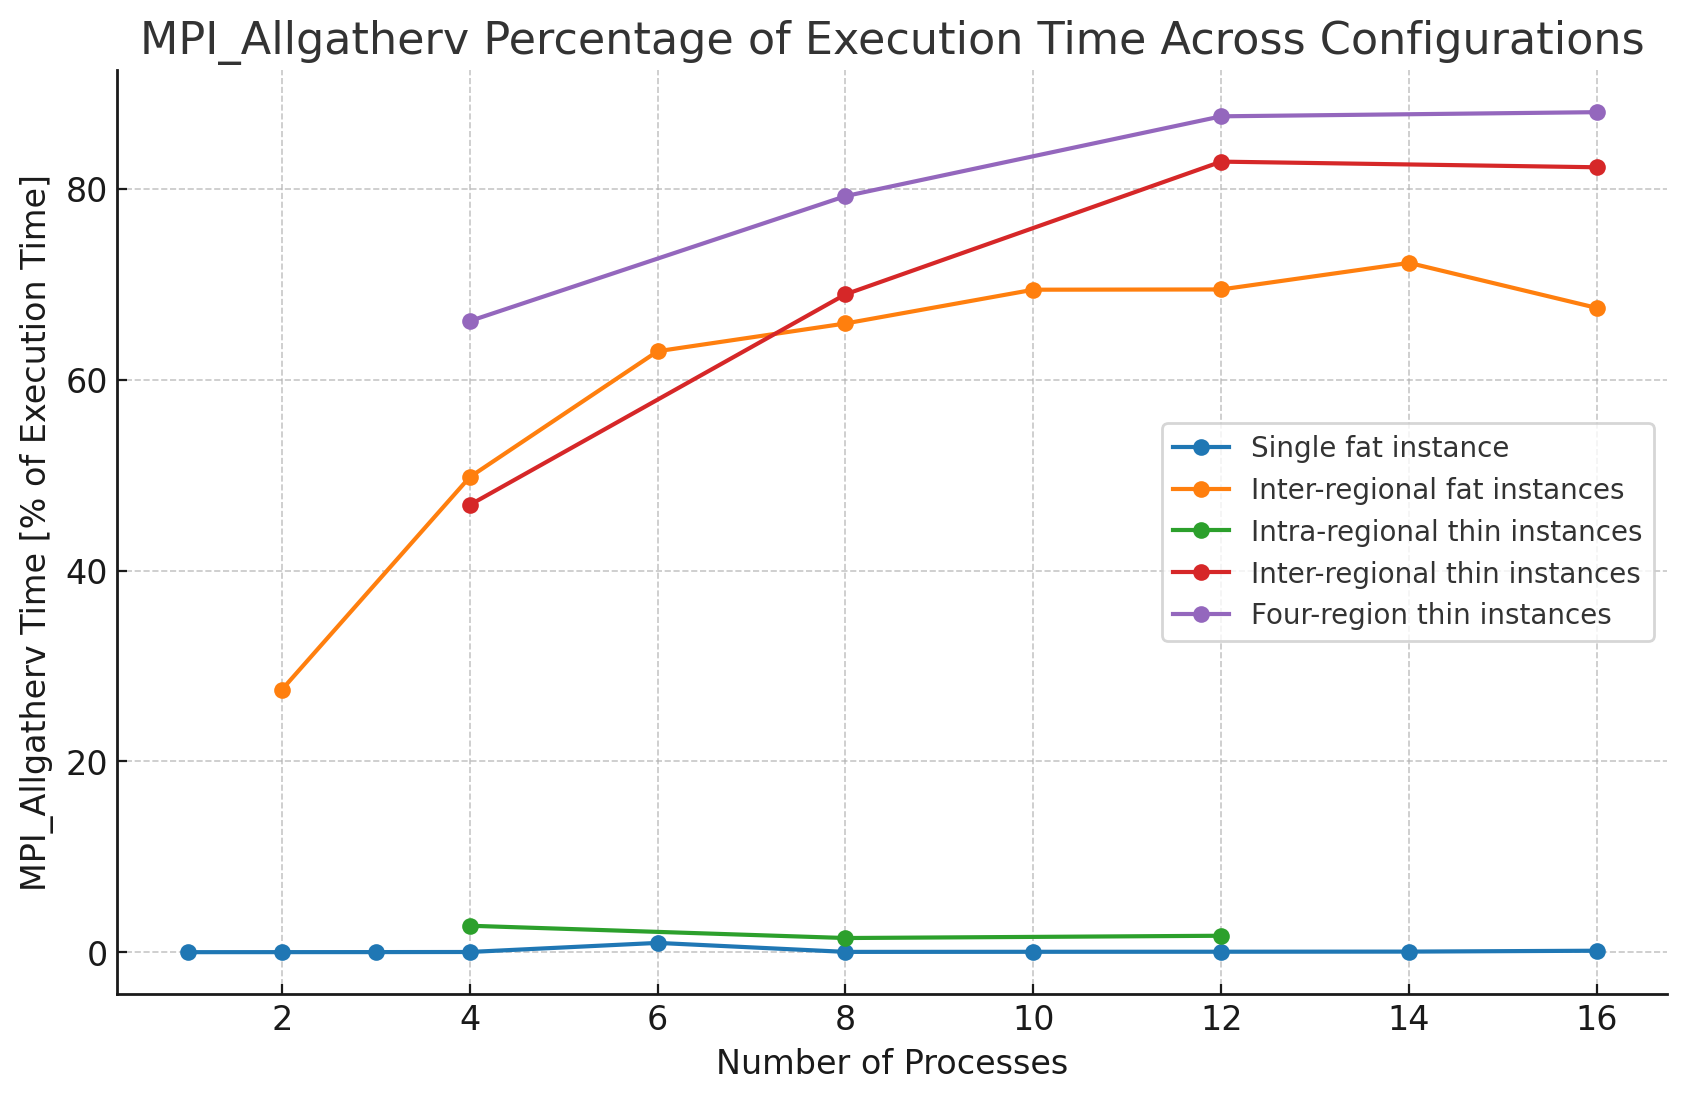
\includegraphics[width=0.8\linewidth]{communication_fraction_ex_time.png}
\caption{Percentage of execution time spent in \texttt{MPI\_Allgatherv} across all GCP configurations.}
\label{fig:comparison_fraction_communication}
\end{figure}

\begin{figure}[H]
\centering
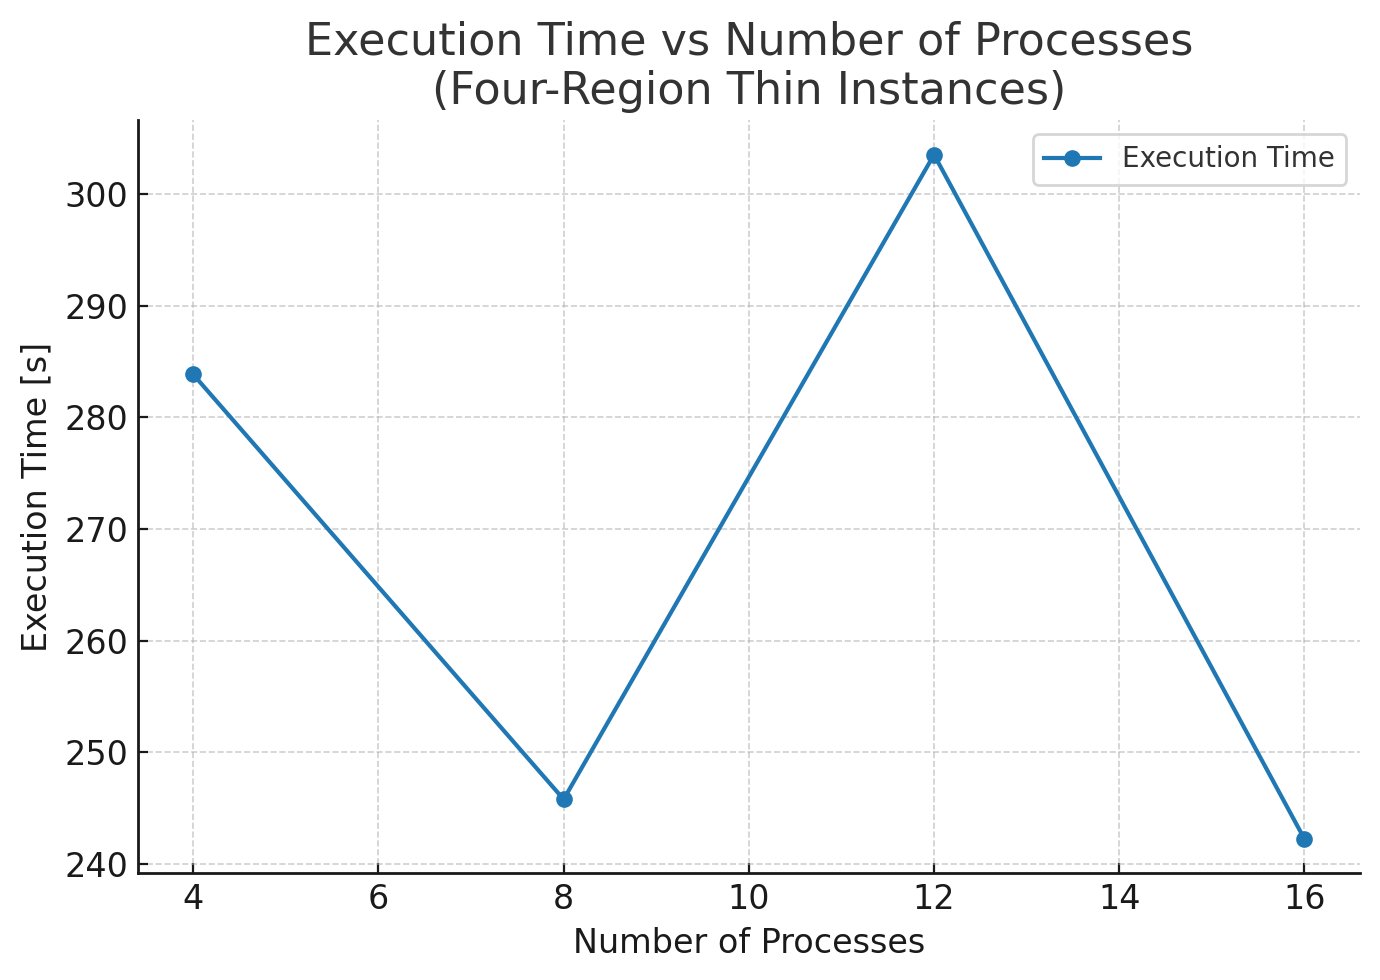
\includegraphics[width=0.8\linewidth]{four_region_ex_time.png}
\caption{Execution times of the four-region cluster: communication overhead dominates, leading to poor strong scalability.}
\label{fig:four_region_ex_time}
\end{figure}

\subsubsection{Weak Scalability Analysis}
As proved in Subsection~\ref{subsec:theoretical_scalability}, the per-process workload grows with $P$, thus the overall execution time of the parallel application increases rather than staying constant.
Rearraging equation~\ref{eq:scalability} we obtain:
\begin{equation}
t_{parallel}(P) = P\times t_{parallel}(1)
\end{equation}
Hence, when doubling both the number of processes and the number of bodies, the running time is expected to double as well, which is exactly what is observed in Figure~\ref{fig:empirical_weak_scalability}.
Further consideration of other configurations beyond the single fat instance is unnecessary, because the weak scalability performance can only worsen due to the communication overhead.

Unfortunately, this is an inherent limitation of the direct method formulation in the N-Body problem.
The simplest way to improve weak scalability is to relax the physics by neglecting the influence of distant (non-local) bodies. This reduces the inner loop (Algorithm~\ref{alg:parallel_inner_loop} complexity to $O((\frac{N}{P})^2)$ which would make constant the per-process workload.

More scalable approaches involve switching to approximate or hierarchical algorithms such as Barnes–Hut or Particle Mesh, which reduce the computational complexity from $O(N^2)$ to $O(N \log N)$ or even $O(N)$, while maintaining acceptable physical accuracy. For a practical comparison of these techniques, see Blelloch and Narlikar~\cite{blelloch1997practical}.

\begin{figure}[H]
\centering
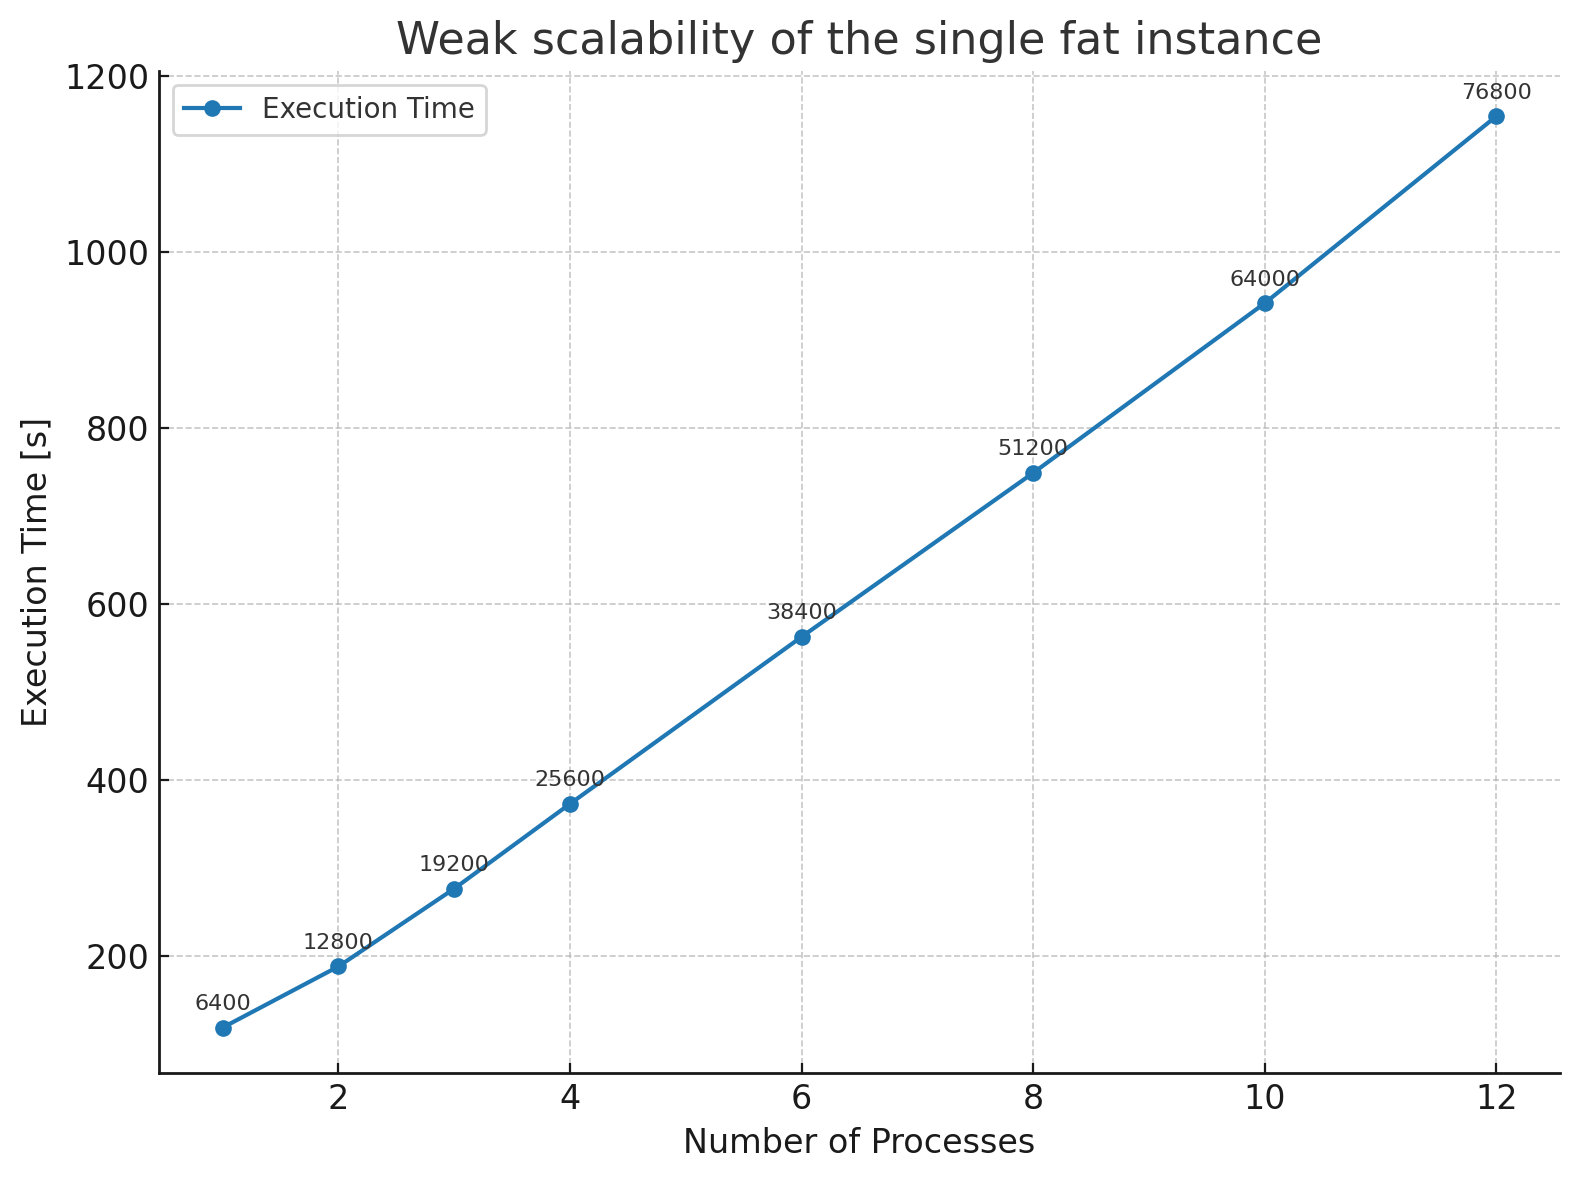
\includegraphics[width=0.8\linewidth]{parallel_weak_scalability.png}
\caption{The parallel application exhibits a very poor weak scalability.}
\label{fig:empirical_weak_scalability}
\end{figure}



\appendix


\section[Simulation Parameters (Solar System)]{Simulation Parameters for the Solar System Test}
\label{appendix:solar_params}

The following configuration was used for the simulation shown in Figure~\ref{fig:long_solar_system}:

\begin{verbatim}
39.4784176 10 20000 0.001
1.0
0 0 0
0 0 0
3.00e-6
0.39 0 0
0 10.2 0
3.26e-7
0.72 0 0
0 7.4 0
3.00e-6
1.0 0 0
0 6.28 0
3.32e-7
1.52 0 0
0 5.1 0
9.50e-4
5.2 0 0
0 2.75 0
2.86e-4
9.58 0 0
0 2.03 0
4.36e-5
19.2 0 0
0 1.43 0
5.15e-5
30.1 0 0
0 1.14 0
1.02e-8
39.5 0 0
0 1.0 0
\end{verbatim}

Where the first line specifies:
\begin{itemize}
    \item Gravitational constant $G$
    \item Number of bodies $N$
    \item Number of steps $T$
    \item Time step $\Delta t$
\end{itemize}
and each body is defined by: mass, initial $(x, y, z)$ position, and initial $(v_x, v_y, v_z)$ velocity.

\section[Machine Specifications]{Machine Specifications}
\label{appendix:machine_specs}

\begin{verbatim}
Architecture       x86_64
CPU Model          AMD Ryzen 5 5625U
                   with Radeon Graphics 
                   (12 threads, 6 cores)
Base/Max Clock     2.3 GHz / 4.388 GHz
L1 Cache           192 KiB (6 instances)
L2 Cache           3 MiB (6 instances)
L3 Cache           16 MiB (1 instance)
Memory             8 GB DDR4
OS                 Ubuntu 22.04.5 LTS, 64-bit
Compiler           gcc 11.4.0 with
                   -O2 optimization
\end{verbatim}


\section{Serial Implementation Timing Data}
\label{appendix:serial_times}
The following table reports the execution times (in seconds) measured for the performance analysis in Subsection~\ref{subsec:num_int}.

\begin{table}[H]
    \centering
    \begin{tabular}{r r}
        \toprule
        \textbf{$N$ (bodies)} & \textbf{Execution time (s)} \\
        \midrule
        100 & 0.012 \\
        200 & 0.049 \\
        400 & 0.198 \\
        800 & 0.796 \\
        1600 & 3.187 \\
        3200 & 12.732 \\
        6400 & 50.902 \\
        12800 & 203.671 \\
        \bottomrule
    \end{tabular}
    \caption{Execution times used to generate Figures~\ref{fig:ex_time} and~\ref{fig:logex_time}.}
    \label{tab:serial_times}
\end{table}

\section{Profiling Results}
\label{appendix:profiling_results}
This appendix reports profiling data for the serial C implementation.
Two profiling tools were used:
\begin{itemize}
    \item GNU \emph{gprof}, to obtain a function-level breakdown of execution time.
    \item Linux \emph{perf}, to collect low-level CPU performance metrics.
\end{itemize}

\subsection{gprof Flat Profile (Summary)}
\label{appendix:gprof_results}
The program was compiled with the \texttt{-pg} flag and executed under the same settings used in the performance analysis (\S\ref{subsec:num_int}) with the exception of $N = 10000$. The resulting \texttt{gmon.out} file was processed with:
\begin{verbatim}
gprof serial gmon.out > profiling_report.txt
\end{verbatim}
\begin{table}[H]
\centering
\label{tab:gprof_summary}
\begin{tabular}{lrrr}
\toprule
\textbf{Function} & \textbf{\% Time} & \textbf{Self (s)} & \textbf{Calls}  \\
\midrule
\texttt{computeAccelerations} & 98.49 & 150.54 & 100 \\
\texttt{\_init}               &  1.49 &   2.28 & --- \\
\texttt{computeVelocities}    &  0.01 &   0.02 & 100 \\
\texttt{logPositions}         &  0.01 &   0.01 & 101 \\
\texttt{rand\_uniform}        &  0.00 &   0.00 & 60000 \\
\texttt{computePositions}     &  0.00 &   0.00 & 100 \\
\texttt{simulate}             &  0.00 &   0.00 & 100 \\
\texttt{initiateSystem}       &  0.00 &   0.00 & 1   \\
\bottomrule
\end{tabular}
\caption{Distribution of execution time by function (gprof flat profile).}
\end{table}
Please note that the \texttt{\_init} function is not part of the N-body program; it is automatically inserted by the C runtime environment during the executable’s startup sequence to perform system-level 
initializations before \texttt{main()} is called.


\subsection{perf Results}
\label{appendix:perf_results}
The profiling command used was:
\begin{verbatim}
perf stat ./serial 12800
\end{verbatim}

\begin{verbatim}
 Task-clock (ms)          268.400
 
 CPU Utilization          1.000 CPUs

 Context-switches         933     (3.48/s)
 
 CPU Migrations           194     (0.72/s)

 Page-faults              316     (1.18/s)

 Cycles                   1.165e9 (4.341 GHz)

 Stalled-cycles-frontend  1.590e6
                          (0.14% frontend idle)

 Instructions             2.837e9 (2.43 IPC)

 Branches                 1.152e8

 Branch-misses            7.05e7
                         (0.06% of all branches)

 Elapsed time (s)         268.410

 User time (s)            268.398

 System time (s)          0.002
\end{verbatim}

\section{GCP Experiments Data}
\label{appendix:gcp_data}
\subsection{Measurement Methodology}
The execution and communication times reported in this appendix were measured using the 
\texttt{MPI\_Wtime()} function, which returns the elapsed wall-clock time in seconds. 
Specifically, timestamps were recorded immediately before and after the code sections of interest, 
and their difference was accumulated across iterations.
For instance, the cumulative time spent in the \texttt{MPI\discretionary{}{}{}Allgatherv} routine was measured as follows:
\begin{lstlisting}
t7 = MPI_Wtime();
MPI_Allgatherv(local_positions, b, MPI_VECTOR, global_positions, recvcounts, displs,MPI_VECTOR, MPI_COMM_WORLD);
t8 = MPI_Wtime();
cumul_time_allgatherv3 += t8 - t7;
\end{lstlisting}

\subsection{Single Fat Instance}
\begin{verbatim}
#Proc   ExecTime[s]   CommTime[s]
1       453.49        0.003
2       231.26        0.010
3       146.31        0.012
4       110.36        0.021
6       75.06         0.730
8       56.97         0.017
10      45.58         0.018
12      38.38         0.018
14      33.38         0.020
16      29.62         0.045
\end{verbatim}

\subsection{Inter-regional Fat Instances}
\begin{verbatim}
#Proc   ExecTime[s]   CommTime[s]
2       258.13        71.01
4       190.75        94.97
6       174.07        109.63
8       146.50        96.53
10      131.86        91.55
12      111.25        77.27
14      108.22        78.18
16      81.08         54.74
\end{verbatim}

\subsection{Intra-regional Thin Instances}
\begin{verbatim}
#Proc   ExecTime[s]   CommTime[s]
4       96.00         2.66
8       48.58         0.72
12      32.55         0.56
\end{verbatim}

\subsection{Inter-regional Thin Instances}
\begin{verbatim}
#Proc   ExecTime[s]   CommTime[s]
4       179.09        83.94
8       163.20        112.52
12      213.73        177.08
16      157.28        129.38
\end{verbatim}

\subsection{Four-region Thin Instances}
\begin{verbatim}
#Proc   ExecTime[s]   CommTime[s]
4       283.83        187.73
8       245.79        194.76
12      303.51        265.88
16      242.24        213.26
\end{verbatim}

\subsection{Weak Scalability (Single Fat Instance)}
\begin{verbatim}
#Proc   #Bodies   ExecTime[s]
1       6400      118.98
2       12800     188.44
3       19200     276.88
4       25600     373.24
6       38400     562.96
8       51200     749.22
10      64000     942.11
12      76800     1154.50
\end{verbatim}






\bibliographystyle{IEEEtran} %I had to install a package through the package manager to use 'IEEEtran'.
\bibliography{refs} 
\end{document}
